% ***********************************************
%***********COSAS A MEJORAR O CORREGIR***********
%	
%
%
%
%
%
%
% ***********************************************
% Preamble
% ---
\documentclass[10pt,a4paper]{article}

% Packages
% ---
\usepackage[latin1]{inputenc}
\usepackage{amsmath}
\usepackage{mathtools}
\usepackage{amsfonts}
\usepackage{amssymb}
\usepackage{layout}
\usepackage{graphics}
\usepackage{graphicx}
\usepackage[spanish]{babel}
\usepackage{lastpage}
\usepackage{tabto}
\usepackage{xcolor,colortbl}
\usepackage{verbatim}
\usepackage[a4paper, top=1 in,bottom=1in, left=1 in, right=0.7 in]{geometry}
\usepackage{fancyhdr}
\pagestyle{fancy}
\usepackage{comment}
\usepackage{bigints}
\usepackage{tikz}
\usepackage{pgfplots}
\pgfplotsset{width=12cm,height=4cm,compat=1.15}


\usetikzlibrary{calc}
\usepackage{gnuplottex}
\usepackage{extarrows}
\usepackage{mathrsfs}


\newtheorem{teorema}{Teorema}

%\usetikzlibrary{circuits,arrows,positioning}

\usepackage[export]{adjustbox}

%ELEGIR VERSION 
%Comentar para eliminar la solucion de todos los ejercicios y dejar la version para los 
% alumnos, a saber con un solo punto resuelto por ejercicio.

\includecomment{profesor}    % version profesor
%\excludecomment{profesor}	  % version alumnos

\lhead{\footnotesize An\'alisis de Se\~nales y Sistemas  - A\~no \the\year{} Ver. 2022.09.15}\chead{}
\rhead{\footnotesize Trabajo Pr\'actico N$^\text o$8: Muestreo y análisis de Fourier en tiempo discreto}
\lfoot{}
\cfoot{}
\rfoot{\footnotesize P\'agina \thepage\ de \pageref{LastPage}}
\renewcommand{\headrulewidth}{0.4pt}
\renewcommand{\footrulewidth}{0.4pt}

\title{
	\textsc{
\includegraphics[width=0.55\textwidth]{logoUTN.jpg}} ~\\
	{\large Departamento de Electr\'onica}\\ 
	[0.1cm]
	{\Huge{An\'alisis de Se\~nales y Sistemas}} \\
	[0.25cm]
	{\Large{Trabajo Pr\'{a}ctico N$^{\text {o}}$8: Muestreo y análisis de Fourier en tiempo discreto}		
	\\
	}}
\author{}
\date{}


% Main document ********************************************
% ---
\begin{document}
\maketitle
\begin{profesor}
	\hspace{6cm}(Versión PROFESOR)
\end{profesor}
\thispagestyle{fancy}

\section*{Enunciados:}
\label{sec:enun}

\begin{enumerate}
\subsubsection*{Muestreo}
% ***********************************************
% 					Ejercicio 1
% ***********************************************
\item {Dadas las siguientes señales, adoptar una frecuencia útil de muestreo y determinar el intervalo $\Delta t$ 
correspondiente:}
\begin{enumerate}
\item $x(t)=10\cos(5t)-5\sin(7\pi t)+3\cos(30t)$ **				
\item $y(t)=18\sin(10t)+15\sin(5\pi t)+5\cos(60t)$
\item $z(t)=15\cos(6\pi t)+7\sin(10\pi t)+2\cos(15\pi t)$			
\end{enumerate}	

% ***********************************************
% 					Ejercicio 2
% ***********************************************
\item {Representar las componentes de los ejemplos anteriores en el eje $\Omega$ y luego calcular $\omega_4$ para 
$\Omega_4=\pi/2$.~~**}

% ***********************************************
% 					Ejercicio 3
% ***********************************************
\item {Para la señal $z(t)$ del ejercicio 1, se adopta $\omega_s=80~rad/s$}.~~**
\begin{enumerate}
	\item Determinar el efecto que se produce				
	\item ¿Cuál es la porción de la señal bien muestreada?
	\item ¿Se produce deterioro? ¿Qué frecuencia o frecuencias se pierden?
	\item ¿Cuál es la frecuencia ``alias'' de la componente mal muestreada?			
\end{enumerate}	

% ***********************************************
% 					Ejercicio 4
% ***********************************************
\item {Una señal $x(t)$ ha sido recuperada por sus muestras obtenidas con una frecuencia de muestreo 
$\omega_s=5000\pi$. ¿Para qué valores de $\omega$ debe garantizarse que $X(j\omega)$ sea cero?}.~~**

% ***********************************************
% 					Ejercicio 5
% ***********************************************
\item {Sea una señal $x(t)$ tal que $X(j\omega)$ tiene el espectro (A) que se muestra en la Fig.~\ref{fig:ej_5}. Se 
suma ruido con espectro (B). Suponiendo que 	$\omega_{max}=1.000~rad/s$; $\omega_{1}=1.500~rad/s$; 
$\omega_{2}=2.000~rad/s$; proponer dos formas de realizar el muestreo sin afectar el espectro (A) de la señal.}~~**

\begin{figure}[h]
	\begin{center}
		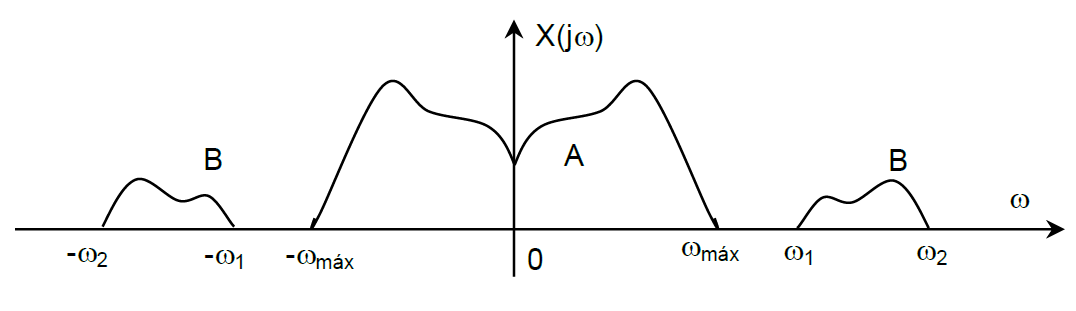
\includegraphics[width=12cm]{tp8_ej5.png}
	\end{center}
	\caption{Gráfica del ej. 5}
	\label{fig:ej_5}
\end{figure}

% ***********************************************
% 					Ejercicio 6
% ***********************************************
\item {Suponer que $x(t)$ tiene por espectro a $X(j\omega)$, que se muestra en la Fig.~\ref{fig:ej_6}. Si se adopta una 
frecuencia de muestreo de $f_s=150~Hz$, ¿qué porción del espectro presenta solapamiento?. Graficar el espectro 
resultante. ¿Cómo se ve la componente $\omega=460~rad/s$?}.

\begin{figure}[h]
	\begin{center}
		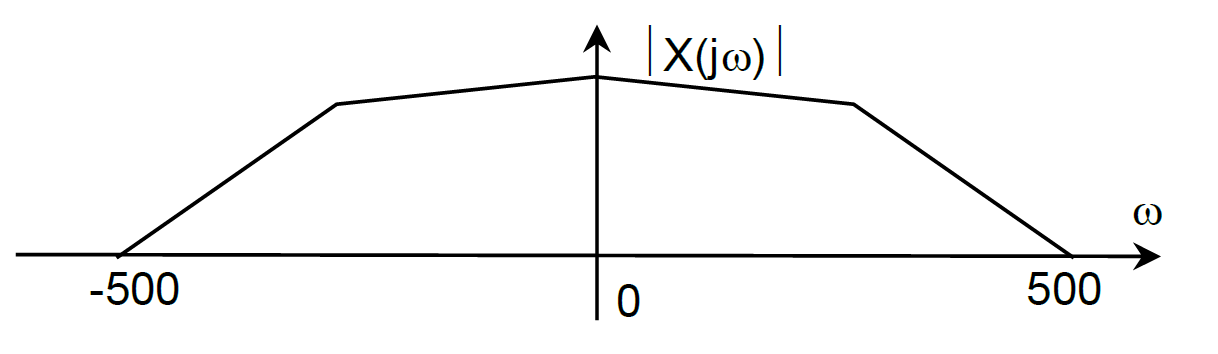
\includegraphics[width=8cm]{tp8_ej6.png}
	\end{center}
	\caption{Gráfica del ej. 6}
	\label{fig:ej_6}
\end{figure}

% ***********************************************
% 					Ejercicio 7
% ***********************************************
\item {Un sistema puede realizar la operación de muestreo con un período mínimo $\Delta t_{min}=1~\mu s$. ¿Qué valores 
puede tomar $\omega_{max}$?}.

% ***********************************************
% 					Ejercicio 8
% ***********************************************
\item {Una señal de audio abarca de $20~Hz$ hasta $20~kHz$. Muestrearla y representarla en $\Omega$.}

% ***********************************************
% 					Ejercicio 9
% ***********************************************
\item {Una señal de RF tiene componentes desde $992~kHz$ hasta $1008~kHz$}.
\begin{enumerate}
	\item Muestrearla y representarla en $\Omega$			
	\item Comparar la gráfica con la del ejercicio 8
	\item ¿Cuánto representa $\Omega=\pi/3$ en cada caso?			
\end{enumerate}	

% ***********************************************
% 					Ejercicio 10
% ***********************************************
\item {El espectro de una señal de voz es prácticamente nulo a frecuencias superiores de $5~kHz$.}~~**
\begin{enumerate}
	\item Determinar la frecuencia y el intervalo de Nyquist.		
	\item Proponer una frecuencia de utilidad práctica para el muestreo.
	\item Graficar el espectro de amplitud de la señal en función de $\Omega$ después del muestreo.
	\item Si el espectro de la señal muestreada tiene una componente en $\Omega=1.75~rad$, ¿cuál es su correspondiente 
	frecuencia $\omega$?
	\item Analizar qué sucede si se elige la frecuencia de muestreo de $8~kHz$.
\end{enumerate}	
	
\subsubsection*{Serie de Fourier para señales en tiempo discreto}

% ***********************************************
% 					Ejercicio 11
% ***********************************************
\item {Para la señal periódica discreta $x[n]$, tal que $x[n]=1$ para $-1 \leq n \leq 2$ y $N=10$, determinar:}~~**
\begin{enumerate}
	\item La serie de Fourier		
	\item Módulo y fase de $a_k$
	\item Las gráficas correspondientes al módulo y la fase de $a_k$
\end{enumerate}	

% ***********************************************
% 					Ejercicio 12
% ***********************************************
\item {Para la señal periódica discreta $x[n]$, tal que $x[n]=0.7^n$ para $0 \leq n \leq 4$ y $N=5$, determinar:}
\begin{enumerate}
	\item La serie de Fourier		
	\item Módulo y fase de $a_k$
	\item Las gráficas correspondientes al módulo y la fase de $a_k$
\end{enumerate}

\subsubsection*{Transformada de Fourier para señales en tiempo discreto}
% ***********************************************
% 					Ejercicio 13
% ***********************************************
\item {Dada la señal transitoria $x[n]$, obtener y graficar $|X(e^{j\Omega})|$:}~~**
\begin{enumerate}
	\item $x[n]=\{3\quad 2\quad 1\quad 0\quad -1\}$
	\item $x[n]=\{-2\quad -1\quad 3\quad 1\}$
\end{enumerate}	

\end{enumerate}
% ***********************************************
% 			Herramientas Teóricas (HT)
% ***********************************************

% *** PAUTAS A SEGUIR ***
\begin{comment}
Esta sección esta pensada para incluir toda la ayuda teórica necesaria 
para resolver el practico.
Algunas reglas generales:
	-Mantener el contenido al minimo, referir a la bibliografía para mayor 
		información (hay q armar un archivo .bib).
	-Enumerar todas las ecuaciones.
	-No repetir ecuaciones ya dadas en las HT de otro práctico, 
		solo referir a ella.
	-Para resaltar palabras usar \textit.
	-Utilizar la nomencaltura oficial de la catátedra !!  
		(Hay que definirlo, yo diria seguir al pie de la letra el kreizig)
\end{comment}

% *** CONTENIDO ***
\section*{Herramientas Te\'oricas:}
\label{sec:herr}

%%%%%%%%%%%%%%%%%%%%%%%%%%%%%%%%%%%%%%%%%%%%%	
\subsection*{Teorema de muestreo}
Sea $x(t)$ una señal de banda limitada, es decir que se cumple: $X(j\omega)=0$ para todo $|\omega|>\omega_{max}$. Puede 
determinarse univocamente $x(t)$ a partir de su versión muestreada $x[n]=x(n\Delta t)$ siempre que la frecuencia de 
muestreo $\omega_s=2\pi/\Delta t$ sea 
\begin{equation}\label{eq:teorema_muestreo}
\omega_s>2\omega_{max}.
\end{equation}

%%%%%%%%%%%%%%%%%%%%%%%%%%%%%%%%%%%%%%%%%%%%%	
\subsection*{Frecuencia digital}

Al muestrear una señal de tiempo continuo, tomamos valores de su variable independiente solo 
para múltiplos enteros del periodo de muestreo $\Delta t$. Para el caso de una señal periódica con período $T$, por 
ejemplo un sinusoide, podemos escribir:
\begin{equation}
x(t)=\sin(wt)\to x[n]=\sin(\omega n\Delta t)=\sin(\Omega n)
\end{equation} 
Mientras que para $x(t)$ la variable independiente $t$ tiene unidades de tiempo ($s$) y su frecuencia angular 
$\omega=2\pi/T$ se mide en $rad/s$; para la señal muestreada $x[n]$, la variable independiente es el indice discreto 
adimensional $n$. Para mantener la relación conocida entre tiempo y frecuencia, es conveniente  al trabajar con señales 
periódicas de tiempo discreto, definir una frecuencia digital $\Omega=2\pi/N$ que se mide en $rad$ y cumple la 
siguiente relación,
\begin{equation}
\Omega=\omega \Delta t
\end{equation} 
Como se ilustra en la Fig.~\ref{fig:frec_dig}, la representación en el dominio de la frecuencia de señales de 
tiempo discreto presenta espectros periódicos cada $\omega_s=2\pi/\Delta t$. Al expresar el espectro en función de la 
frecuencia digital, se ve que siempre es periódico cada  $\Omega_{s}=\omega_{s}\Delta t=2\pi~rad$. 

Además, al comparar las amplitudes del espectro de la señal de tiempo continuo $X(j\omega)$, con el de la señal 
muestreada $X(e^{j\Omega})$ obtenido mediante la transformada 
de Fourier de tiempo discreto, se hace manifiesto el factor de escala $1/\Delta t$.

\begin{figure}[h]
	\begin{center}
		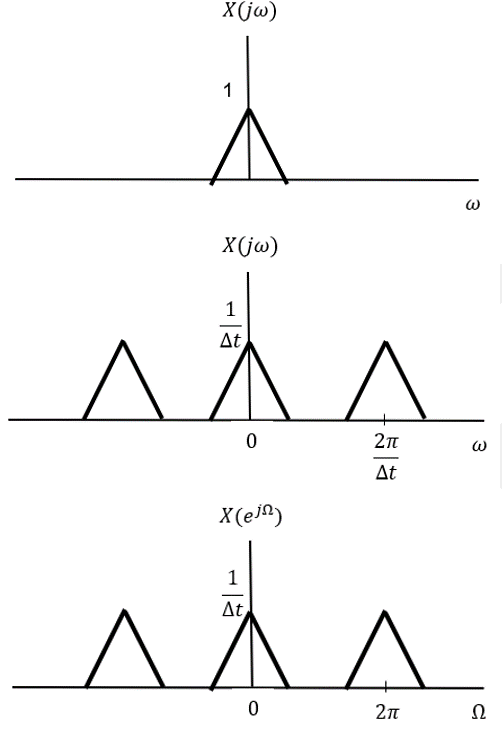
\includegraphics[width=6cm]{frec_dig.png}
	\end{center}
	\caption{Espectro de una señal no periodica de tiempo continuo de banda limitada (superior) y de la misma señal 
		luego de ser 
		muestreada con un intervalo de muestreo $\Delta t$. Este último se muestra tanto en función de la frecuencia 
		angular 
		$\omega$ (centro) como de la 
		frecuencia digital $\Omega$ (inferior).}
	\label{fig:frec_dig}
\end{figure}

%%%%%%%%%%%%%%%%%%%%%%%%%%%%%%%%%%%%%%%%%%%%%	
\subsection*{Serie de Fourier de tiempo discreto}
La ecuación que define a la serie de Fourier para señales de tiempo discreto (a veces llamada serie discreta de Fourier) es,
\begin{equation}
x[n] = \sum_{k=\langle N\rangle} a_k e^{jk\Omega_0n},
\end{equation}
siendo $\Omega_0=2\pi/N$. Y los coeficientes $a_k$ están dados por,
\begin{equation}
a_k = \frac{1}{N} \sum_{n=\langle N\rangle} x[n]e^{-jk\Omega_0n}.
\end{equation}

Notar que a diferencia de las ecuaciones de Fourier para tiempo continuo, la series involucradas aquí son de longitud 
finita $N$ (debido a la periodicidad de los $a_k$). En consecuencia, puede evitarse el truncamiento y sintetizar la 
señal $x[n]$ exactamente a partir de los $N$ coeficientes $a_k$.

%%%%%%%%%%%%%%%%%%%%%%%%%%%%%%%%%%%%%%%%%%%%%	
\subsection*{Transformada de Fourier de tiempo discreto}
La ecuación que define la transformada de Fourier para señales de tiempo discreto no periódicas es,
\begin{equation}
X(e^{j\Omega}) = \sum_{n=-\infty}^{+\infty}x[n]e^{-j\Omega n}.
\end{equation}
Mientras que la transformación inversa es:
\begin{equation}
x[n] = \frac{1}{2\pi} \int_{\langle 2\pi \rangle} X(e^{j\Omega})e^{j\Omega n} d\Omega.
\end{equation}



% ***********************************************
% 					SOLUCIONES
% ***********************************************
% *** PAUTAS A SEGUIR ***
\begin{comment}
En esta sección se resuelven los ejercicios paso a paso.
Algunas reglas generales:
	-Utilizar la resolución mas didáctica posible y 
		que sea consistente con los otros prácticos.
	-Dar la suficiente cantidad de detalle para que sea sencillo
		entender lo que se está haciendo, pero sin caer en trivialidades.
	-Para explicar lo que se hace en un desarrollo, ir comentando a la derecha
		de cada paso, usando usando "\begin{align}" u otro que lo permita
	-Todas las soluciones finales de los ejercicios deben estar recuadradas 
		con \boxed{}
	-Cuando haya que desarrollar partes con jerarquía, usar primero negrita

		y luego cursiva para sub partes.
\end{comment}

% *** DESARROLLO ***
\section*{Soluciones}
\label{sec:sol}

\begin{enumerate}
% ***********************************************
% 					Ejercicio 1
% ***********************************************
\item 
\begin{enumerate}
\item[\textit{b})]
Para poder adoptar una frecuencia útil de muestreo es necesario en primer lugar identificar cuál es la máxima frecuencia de la señal. Observamos que para este caso tenemos las componentes con frecuencias
\begin{align}
\omega_1 &= 10 ~rad/s, \\
\omega_2 &= 5\pi ~rad/s \approx 15.7 ~rad/s, \\
\omega_3 &= 60 ~rad/s,
\end{align}
donde claramente se observa que la máxima frecuencia es $\omega_3 = 60 ~rad/s$. A continuación lo que se debe hacer es determinar una frecuencia de muestreo que cumpla con el teorema de muestreo definido en la Ec. \ref{eq:teorema_muestreo}, la que podría ser por ejemplo,
\begin{equation}
\omega_s = 2.5 \cdot\omega_3 = 150 ~rad/s.
\end{equation}
El intervalo de muestreo para esta $\omega_s$ es
\begin{equation}
\Delta t=\frac{2\pi}{\omega_s}=\frac{2\pi}{150~rad/s}=41.9~ms.
\end{equation}
\end{enumerate}


% ***********************************************
% 					Ejercicio 2
% ***********************************************
\item
La relación entre las variables de frecuencia $\omega$, para tiempo continuo, y $\Omega$, para tiempo discreto, esta dada por
\begin{equation}
\Omega = \omega \Delta t.
\end{equation}

Para cada una de las frecuencias del punto 1.\textit{b}) se tiene
\begin{align}
\Omega_1 &= 10 ~rad/s \cdot 41.9~ms = 0.13\pi ~rad, \\
\Omega_2 &= 5\pi ~rad/s \cdot 41.9~ms = 0.21\pi ~rad, \\
\Omega_3 &= 60 ~rad/s\cdot 41.9~ms = 0.8\pi ~rad.
\end{align}

Para un valor de frecuencia $\Omega_4=\pi/2$ se tiene,
\begin{equation}
\omega_4=\frac{\Omega_4}{\Delta t}=\frac{\pi/2}{41.9ms}\approx 75 ~rad/s.
\end{equation}

\begin{figure}[htb]
	\centering	
	% ___ gráfica
	\begin{tikzpicture}[scale=1]
		\begin{axis}[
		axis y line=center,
		axis x line=middle,
		xmin=-4.2*pi,	xmax=4.2*pi,
		ymin=0,	ymax=25/0.042/2,
		xlabel={$\Omega$},
		ylabel={$|X(e^{j\Omega})|$},
		grid=both,
		grid style={line width=.1pt, draw=gray!40},
    	major grid style={line width=.2pt,draw=gray!60},
		minor tick num=3,
   		cycle list name=mark list,
    	mark size=1.3,
		]
		\addplot+[ycomb,black,thick,line width=.8pt] 
			plot coordinates {
				(-4*pi+0.13*pi,18/0.042/2) (-4*pi+0.21*pi,15/0.042/2) (-4*pi+0.8*pi,5/0.042/2)
				(-2*pi-0.8*pi,5/0.042/2) (-2*pi-0.21*pi,15/0.042/2) (-2*pi-0.13*pi,18/0.042/2)
				(-2*pi+0.13*pi,18/0.042/2) (-2*pi+0.21*pi,15/0.042/2) (-2*pi+0.8*pi,5/0.042/2)
				(-0.8*pi,5/0.042/2) (-0.21*pi,15/0.042/2) (-0.13*pi,18/0.042/2) 
				% Omega positivo
				(0.13*pi,18/0.042/2) (0.21*pi,15/0.042/2) (0.8*pi,5/0.042/2) 
				(2*pi-0.8*pi,5/0.042/2) (2*pi-0.21*pi,15/0.042/2) (2*pi-0.13*pi,18/0.042/2)
				(2*pi+0.13*pi,18/0.042/2) (2*pi+0.21*pi,15/0.042/2) (2*pi+0.8*pi,5/0.042/2)
				(4*pi-0.8*pi,5/0.042/2) (4*pi-0.21*pi,15/0.042/2) (4*pi-0.13*pi,18/0.042/2)
				};
	\end{axis}
	\end{tikzpicture}
	\caption{Gráfico del ej. 2}
\end{figure}


% ***********************************************
% 					Ejercicio 3
% ***********************************************
\item
\begin{enumerate}
\item
Para poder determinar el efecto que produce muestrear la señal con una frecuencia de muestreo $\omega_s =80 ~rad/s$ primero se debe determinar cuál es la frecuencia máxima para la señal considerada. Se puede identificar fácilmente que la frecuencia máxima es $\omega_m=15\pi ~rad/s\approx 47.1 ~rad/s$.

Para realizar un muestreo apropiado de la señal se debe cumplir el teorema del muestreo, es decir, que la frecuencia de muestreo debe ser mayor que dos veces la máxima frecuencia presente en la señal, lo que claramente vemos que no se cumple, siendo que $2\omega_m=94.2~rad/s$ para este caso. De esta forma, se estará ante una situación de \textbf{submuestreo} o \textbf{aliasing}.

\item
La porción de la señal bien muestreada es la correspondiente al rango de frecuencias donde no se produce solapamiento. 
Esto sería todas las frecuencias por debajo de $\omega_s - \omega_{m} = 32.9~rad/s$

\item
Sí se produce deterioro. Para este caso puntual se pierde la frecuencia $\omega_m=47.1~rad/s$.

\item
La frecuencia ``alias'' de la componente mal muestreada se obtiene como,
\begin{equation}
\omega_{alias}=\omega_s-\omega_m=80~rad/s-47.1~rad/s=32.9~rad/s.
\end{equation}
Comparar este resultado con el del punto 3.b
\end{enumerate}


% ***********************************************
% 					Ejercicio 4
% ***********************************************
\item A resolver por el alumno

% ***********************************************
% 					Ejercicio 5
% ***********************************************
\item
Una forma de realizar el muestreo de forma adecuada sin afectar el espectro (A) es utilizando un filtro pasa-bajos que elimine el espectro (B) de ruido, y adoptar una frecuencia de muestreo adecuada según el espectro (A). 

Como $\omega_{max} = 1000~rad/s$ y $\omega_1=1500~rad/s$, la frecuencia de corte del filtro debería estar entre estas dos frecuencias y la frecuencia de muestreo podría ser por ejemplo,
\begin{equation}
\omega_s = 2.2~\omega_{max} = 2200~rad/s.
\end{equation}

Otra forma de realizar el muestreo sin afectar el espectro (A) sería adoptar una frecuencia de muestreo tal que el espectro de ruido (B) no se superponga con el espectro (A). Se dejan los detalles numéricos al alumno.


% ***********************************************
% 					Ejercicio 6
% ***********************************************
\item La frecuencia angular de muestreo resulta $\omega_s=2\pi f_s=942.48 ~ rad/s$. Calculamos la componente de alias 
para saber si hay solapamiento (aliasing en la frecuencia), 
$\omega_{alias}=\omega_s-\omega_{max}=942.48-500=442.48~rad/s$. 

Debido a que $\omega_{alias}<\omega_{max}$ hay 
solapamiento para toda $442.48~rad/s<\omega<500~rad/s$, como se ve en la Fig.~\ref{fig:ej_6r}. Notar que la 
componente $\omega=460~rad/s$ está en el intervalo de solapamiento, por lo que presenta una amplitud mayor a la real.

\begin{figure}[h]
	\begin{center}
		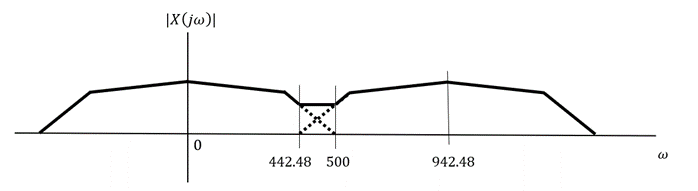
\includegraphics[width=14cm]{tp8_ej6_res.png}
	\end{center}
	\caption{Resolución del ej. 6}
	\label{fig:ej_6r}
\end{figure}

% ***********************************************
% 					Ejercicio 7
% ***********************************************
\item A resolver por el alumno



% ***********************************************
% 					Ejercicio 8
% ***********************************************
\item A resolver por el alumno



% ***********************************************
% 					Ejercicio 9
% ***********************************************
\item A resolver por el alumno



% ***********************************************
% 					Ejercicio 10
% ***********************************************
\item Del enunciado sabemos que el espectro de una señal de voz posee $f_{max}=5~kHz$, a partir de la que 
podemos determinar:
\begin{enumerate}
	\item La frecuencia teórica mínima dada por el teorema del muestreo es la frecuencia de Nyquist, 
	$f_{nyquist}=2f_{max}=10 ~kHz$. El intervalo de Nyquist vale entonces,  
	$\Delta t_{nyquist}=1/f_{nyquist}=100~\mu s$
	\item Para facilitar la implementación del filtro pasa-bajos que permita recuperar la señal a partir de su versión 
	muestreada, se aconseja tomar una frecuencia de muestreo mayor que la de Nyquist. Elegimos,  
	$f_{s}=2.5f_{max}=12.5~kHz$, que resulta en un intervalo de muestreo $\Delta t_s=80~\mu s$
	\item  Ver la Fig.~\ref{fig:ej_10}, donde $\Omega_{max}=\omega_{max}\Delta t_s=2\pi f_{max}\Delta t_s=0.8\pi~rad$ 
	y 
	$\Omega_{alias}=2\pi (f_{s}-f_{max})\Delta t_s=1.2\pi~rad$. Notar que siempre $\Omega_{s}=2\pi f_{s}\Delta 
	t_s=2\pi~rad$.
	\item La frecuencia angular correspondiente a $\Omega=1.75~rad$ es $\omega=\Omega/\Delta t_s= 21.875~rad/s$
	\item Si se elije una frecuencia de muestreo $f_s=8~kHz$, se producirá perdida de información (aliasing), pues no 
	se cumple con el teorema del muestreo. En particular, toda la información contenida en frecuencias mayores a la de  
	alias, $f_{alias}=f_s-f_{max}=3~kHz$, resulta destruida debido al solapamiento de los espectros (se deja al alumno 
	la representación gráfica de este caso). 
\end{enumerate} 

\begin{figure}[h]
	\begin{center}
		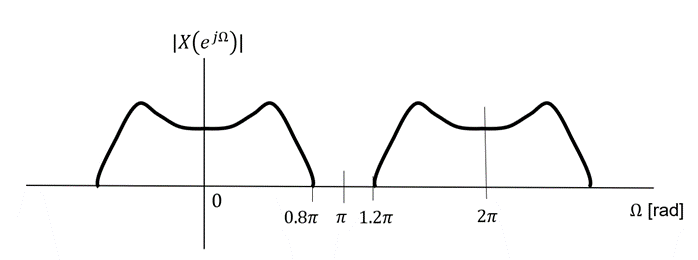
\includegraphics[width=14cm]{tp8_ej10.png}
	\end{center}
	\caption{Resolución del ej. 10}
	\label{fig:ej_10}
\end{figure}


% ***********************************************
% 					Ejercicio 11
% ***********************************************
\item A resolver por el alumno


% ***********************************************
% 					Ejercicio 12
% ***********************************************
\item 
\begin{enumerate}
	\item Calculamos los coeficientes de la serie de Fourier de tiempo discreto para la señal: $x[n]=0.7^n$ para 
	$0\leq n\leq 4$ con periodo $N=5$. Notar que $\Omega_0=2\pi/N=2\pi/5$:
	\begin{align}
	a_k &= \frac{1}{N} \sum_{n=\langle N\rangle} x[n]e^{-jk\Omega_0n},\\
	&= \frac{1}{5} \sum_{n=\langle 5\rangle} 0.7^n e^{-jk\frac{2\pi}{5}n},\\
    &= \frac{1}{5} \sum_{n=\langle 5\rangle} \Big( 0.7 e^{-jk\frac{2\pi}{5}} \Big) ^n.
   	\end{align}
	Que es una serie geométrica, por lo que su suma puede escribirse:
	\begin{align}
	a_k  &= \frac{1}{5}\frac{1-0.7^5}{1-0.7e^{-jk\frac{2\pi}{5}}},\\
	 &=\boxed{\frac{0.1664}{1-0.7e^{-jk\frac{2\pi}{5}}}}.
	\end{align}	
	 Por lo que el desarrollo en serie de Fourier queda:
	\begin{equation}
	x[n] = \sum_{k=\langle 5\rangle} \frac{0.1664}{1-0.7e^{-jk\frac{2\pi}{5}}} e^{jk\frac{2\pi}{5}n},
	\end{equation}
	\item Debido a que solo hay $N=5$ coeficientes diferentes, podemos calcularlos numéricamente en forma polar, por 
	ejemplo:
	\begin{itemize}
		\item $a_0=\frac{0.1664}{1-0.7e^{-j0\frac{2\pi}{5}}}=\frac{0.1664}{1-0.7}=0.5546+0i=0.55e^{j0}$
		\item $a_1=\frac{0.1664}{1-0.7e^{-j1\frac{2\pi}{5}}}=0.1618e^{-j0.7042}$
		\item $a_2=\frac{0.1664}{1-0.7e^{-j2\frac{2\pi}{5}}}=0.1027e^{-j0.2569}$
		\item $a_3=\frac{0.1664}{1-0.7e^{-j3\frac{2\pi}{5}}}=0.1027e^{j0.2569}$
		\item $a_4=\frac{0.1664}{1-0.7e^{-j4\frac{2\pi}{5}}}=0.1618e^{j0.7042}$						
	\end{itemize}
	\item Ver Fig.~\ref{fig:ej_12}.
	\begin{figure}[h]
		\begin{center}
			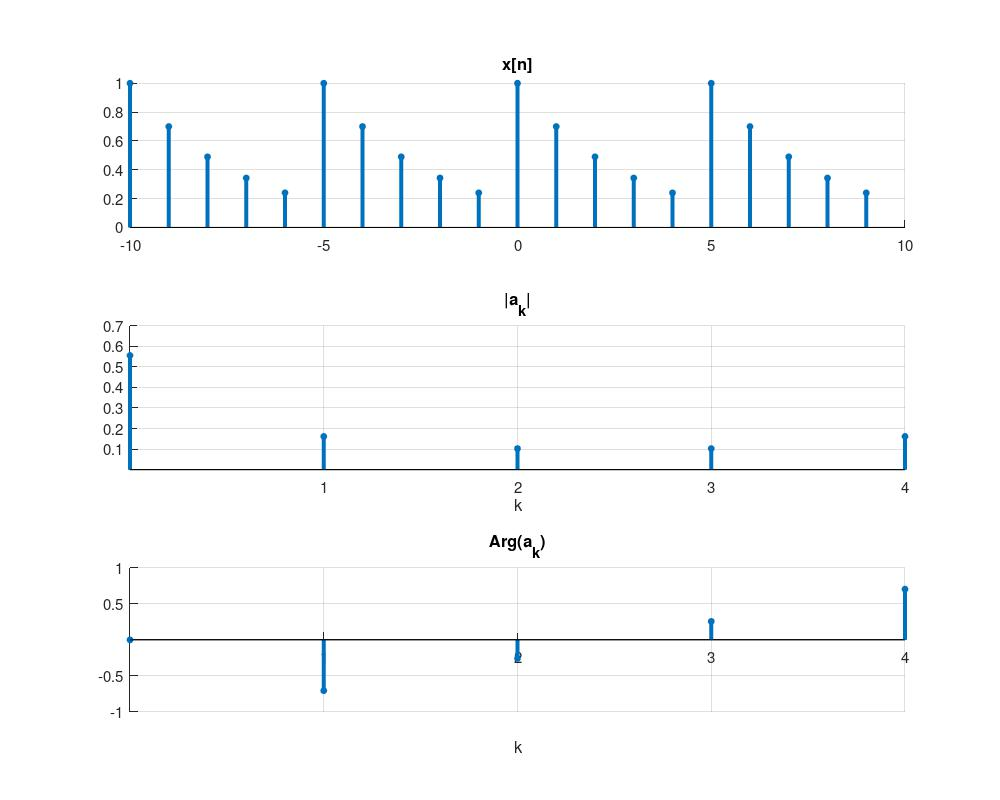
\includegraphics[width=16cm]{tp8_ej12.jpg}
		\end{center}
		\caption{Resolución del ej. 12}
		\label{fig:ej_12}
	\end{figure}
	
\end{enumerate}



% ***********************************************
% 					Ejercicio 13
% ***********************************************
\item
\begin{enumerate}
\item Para obtener la transformada de Fourier de una señal no periódica de duración finita como la dada, 
$x[n]=\{3\quad 2\quad 1\quad 0 \quad -1\}$, aplicamos la definición y resolvemos la suma numéricamente:
\begin{align}
X(e^{j\Omega}) &= \sum_{n=-\infty}^{+\infty}x[n]e^{-j\Omega n}\\
&= \sum_{n=0}^{4}x[n]e^{-j\Omega n}\\
&= \boxed{3+2e^{-j\Omega}+e^{-j\Omega 2}-e^{-j\Omega 4}}.
\end{align}
La señal y su transformada se muestran en la Fig.~\ref{fig:ej_13a}.
\begin{figure}[h]
	\begin{center}
		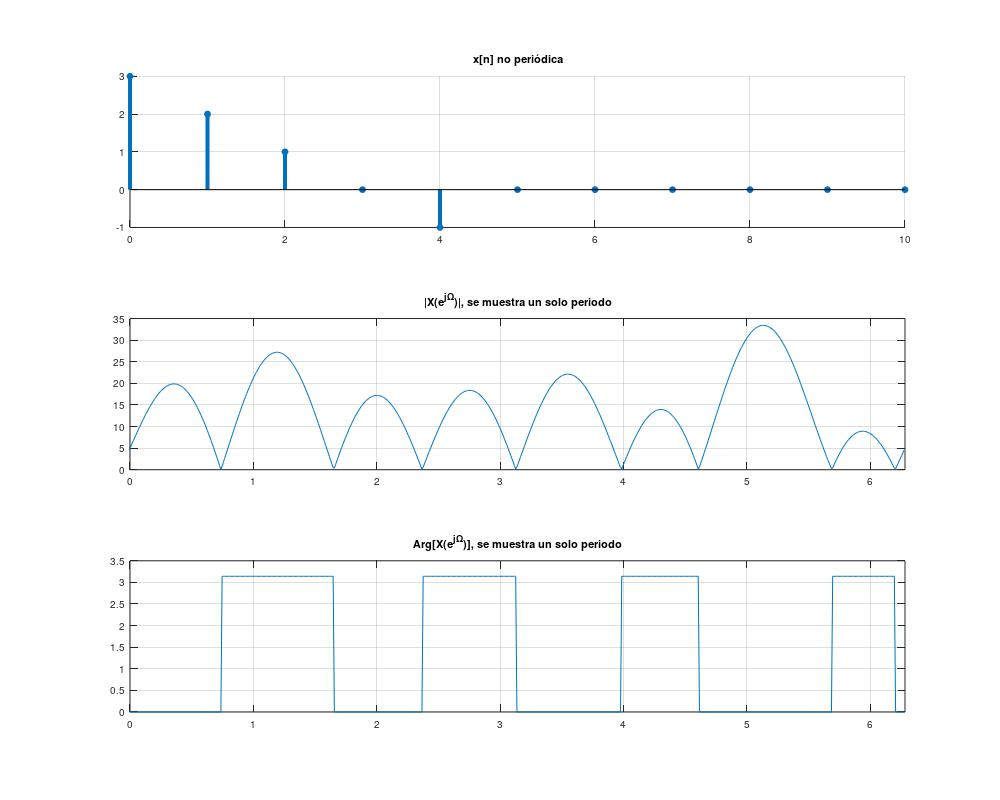
\includegraphics[width=16cm]{tp8_ej13a.jpg}
	\end{center}
	\caption{Resolución del ej. 13a. Notar que se muestra un solo periodo de los espectros.}
	\label{fig:ej_13a}
\end{figure}

\begin{profesor}
	\item Para obtener la transformada de Fourier de una señal no periódica de duración finita como la dada, 
	$x[n]=\{-2\quad -1\quad 3\quad 1\}$, aplicamos la definición y resolvemos la suma numéricamente:
	\begin{align}
	X(e^{j\Omega}) &= \sum_{n=-\infty}^{+\infty}x[n]e^{-j\Omega n}\\
	&= \sum_{n=0}^{3}x[n]e^{-j\Omega n}\\
	&= \boxed{-2-e^{-j\Omega}+3e^{-j\Omega 2}+e^{-j\Omega 3}}.
	\end{align}
\end{profesor}
\end{enumerate}


\end{enumerate}
\begin{center}
---------------------------------------
\end{center}
\end{document}
